In the first experiment, we investigate the impact of three different dead-end handling strategies on the Gini coefficient of PageRank values across various types of graphs. In the second experiment, we attempt six different deterministic heuristics for adding edges to the graph for minimization of Gini coefficient of PageRank values. Dataset for the experiments are obtained from the \href{https://sparse.tamu.edu}{\textit{SuiteSparse Matrix Collection}} \cite{suite19}. Our experiments are reproducible. The codebase is available at our repository.\footnote{https://github.com/puzzlef/pagerank-minimize-inequality}




\subsection{Reading Edgelist from text file}

In this experiment we study the \textbf{Lorenz curve} and \textbf{Gini coefficient} of \textbf{PageRank values} on a number of graphs, and compare between PageRank values obtained with three different \textbf{dead-end handling strategies}: \textit{teleport from dead-ends} (\textbf{default}), \textit{self-loop dead-ends} (\textbf{loop}), and \textit{self-loop all vertices} (\textbf{loopall}). The PageRank values of vertices in each graph is obtained with \href{https://www.npmjs.com/package/nvgraph.sh}{\textit{nvgraph.sh}} \cite{sahu2021nvgraph}, which internally uses \href{https://docs.nvidia.com/cuda/archive/10.0/nvgraph/index.html#nvgraph-pagerank-example}{\textit{nvGraph PageRank}} \cite{nvidia2018nvgraph}. The Lorenz curve of ranks is obtained by sorting the ranks in ascending order and cumulatively summing them up to obtain $100$ samples. These $100$ samples are then compared with the ideal (total equality) Lorenz curve to obtain the Gini coefficient. Note that this is output into YAML files by \textit{nvgraph.sh} itself. This measurement process of Lorenz curve and Gini coefficient is repeated for \textit{loop} and \textit{loopall} variants of graphs, which are generated from the original graph using \href{https://github.com/puzzlef/graph-generate}{\textit{graph-generate}} \cite{sahu2022github}. Finally we process all YAML files into CSV, separately for Gini coefficient and Lorenz curve, and compare the results.

\begin{algorithm}[hbtp]
\caption{Reading Edge-list from file.}
\label{alg:el}
\begin{algorithmic}[1]
\Require{$pdegrees$: Per partition vertex degrees (output)}
\Require{$edges$: Per thread sources, targets, and weights of edges (output)}
\Require{$data$: Memory mapped file data}
\Ensure{$counts$: Number of edges read per thread (output)}
\Ensure{$symmetric$: Is graph symmetric?}
\Ensure{$weighted$: Is graph weighted?}
\Ensure{$\beta$: Size of each block that is processed per thread}
\Ensure{$\rho$: Number of partitions for counting vertex degrees}
\Ensure{$t$: Current thread}

\Statex

\Function{getBlock}{$data, i$} \label{alg:frontier--main-begin}
  \State $[d, D] \gets data$
  \State $b \gets d+i$ \textbf{;} $B \gets min(b+\beta, D)$
  \If{$b \neq d$ \textbf{and not} $isNewline(b-1)$}
    \State $b \gets findNextLine(b, D)$
  \EndIf
  \If{$B \neq d$ \textbf{and not} $isNewline(B-1)$}
    \State $B \gets findNextLine(B, D)$
  \EndIf
  \Return{$[b, B]$}
\EndFunction

\Statex
  
\Function{readEdgelist}{$pdegrees, edges, data$}
  \State $counts \gets \{0\}$
  \State $[sources, targets, weights] \gets edges$
  \State $\rhd$ Load edges from text file in blocks of size $\beta$
  \ForAll{$i \in [0, \beta, 2\beta, ... |data|]$ \textbf{in parallel}}
    \State $j \gets counts[t]$
    \State $[b, B] \gets getBlock(data, i)$
    \While{$true$}
      \State $\rhd$ Read an edge from the block
      \State $u \gets v \gets 0$ \textbf{;} $w \gets 1$
      \State $b \gets findNextDigit(b, B)$
      \If{$b = B$} \textbf{break}
      \EndIf
      \State $b \gets parseWholeNumber(u, b, B)$
      \State $b \gets findNextDigit(b, B)$
      \State $b \gets parseWholeNumber(v, b, B)$
      \If{$weighted$}
        \State $b \gets findNextDigit(b, B)$
        \State $b \gets parseFloat(w, b, B)$
      \EndIf
      \State $\rhd$ Make it zero-based
      \State $u \gets u - 1$ \textbf{;} $v \gets v - 1$
      \State $\rhd$ Add the parsed edge to edgelist
      \State $sources[t][j] \gets u$
      \State $targets[t][j] \gets v$
      \If{$weighted$} $weights[t][j] \gets w$
      \EndIf
      \State $atomicAdd(pdegrees[t \bmod \rho][u], 1)$
      \State $j \gets j + 1$
      \State $\rhd$ If graph is symmetric, add the reverse edge
      \If{$symmetric$}
        \State $sources[t][j] \gets v$
        \State $targets[t][j] \gets u$
        \If{$weighted$} $weights[t][j] \gets w$
        \EndIf
        \State $atomicAdd(pdegrees[t \bmod \rho][v], 1)$
        \State $j \gets j + 1$
      \EndIf
    \EndWhile
    \State $counts[t] \gets j$
  \EndFor
  \Return{$counts$}
\EndFunction
\end{algorithmic}
\end{algorithm}

\begin{algorithm}[hbtp]
\caption{Convert Edge-list to CSR.}
\label{alg:csr}
\begin{algorithmic}[1]
\Require{$csr$: Global CSR (output)}
\Require{$pcsr$: Per partition CSR (scratch)}
\Require{$pdegrees$: Per partition vertex degrees (scratch)}
\Require{$edges$: Per thread sources, targets, and weights of edges}
\Require{$counts$: Number of edges read per thread}
\Ensure{$symmetric$: Is graph symmetric?}
\Ensure{$weighted$: Is graph weighted?}
\Ensure{$\rho$: Number of partitions for counting vertex degrees}
\Ensure{$t$: Current thread}

\Statex

\Function{convertToCsr}{$csr, pcsr, pdegrees, edges, counts$}
  \State $[offsets, edgeKeys, edgeValues] \gets csr$ \label{alg:csr--initialize-begin}
  \State $[poffsets, pedgeKeys, pedgeValues] \gets pcsr$
  \State $[sources, targets, weights] \gets edges$ \label{alg:csr--initialize-end}
  \State $\rhd$ Compute offsets
  \ForAll{$p \in [0, \rho)$} \label{alg:csr--poffsets-begin}
    \State $exclusiveScan(poffsets[p], pdegrees[p], |V|+1)$
  \EndFor \label{alg:csr--poffsets-end}
  \State $\rhd$ Populate per-partition CSR
  \ForAll{\textbf{threads in parallel}} \label{alg:csr--pcsr-begin}
    \ForAll{$i \in [0, counts[t])$}
      \State $u \gets sources[t][i]$
      \State $v \gets targets[t][i]$
      \State $j \gets atomicAdd(poffsets[t \bmod \rho][u], 1)$
      \State $pedgeKeys[t \bmod \rho][j] \gets v$
      \If{$weighted$}
        \State $pedgeValues[t \bmod \rho][j] \gets weights[t][i]$
      \EndIf
    \EndFor
  \EndFor \label{alg:csr--pcsr-end}
  \State $\rhd$ Fix per-partition offsets
  \ForAll{\textbf{threads in parallel}} \label{alg:csr--poffsets-fix-begin}
    \If{$t < \rho$}
      \State $memcpy(poffsets[t]+1, poffsets[t], |V|)$
      \State $poffsets[t][0] \gets 0$
    \EndIf
  \EndFor \label{alg:csr--poffsets-fix-end}
  \State $\rhd$ Combine per-partition degrees
  \ForAll{$u \in [0, |V|)$ \textbf{in parallel}} \label{alg:csr--poffsets-combine-begin}
    \ForAll{$p \in [1, \rho)$}
      \State $pdegrees[0][u] +\gets pdegrees[p][u]$
    \EndFor
  \EndFor \label{alg:csr--poffsets-combine-end}
  \State $\rhd$ Compute global offsets
  \State $exclusiveScan(offsets, pdegrees[0], |V|+1)$ \label{alg:csr--offsets-compute}
  \State $\rhd$ Combine per-partition CSR into one CSR
  \ForAll{$u \in [0, |V|)$ \textbf{in parallel}} \label{alg:csr--pcsr-combine-begin}
    \State $j \gets offsets[u]$
    \ForAll{$p \in [0, \rho)$}
      \State $i \gets poffsets[t][u]$
      \State $I \gets poffsets[t][u+1]$
      \ForAll{$i \in [i, I)$}
        \State $edgeKeys[j] \gets pedgeKeys[t][i]$
        \If{$weighted$}
          \State $edgeValues[j] \gets pedgeValues[t][i]$
        \EndIf
        \State $j \gets j + 1$
      \EndFor
    \EndFor
  \EndFor \label{alg:csr--pcsr-combine-end}
\EndFunction
\end{algorithmic}
\end{algorithm}

\begin{figure}[hbtp]
  \centering
  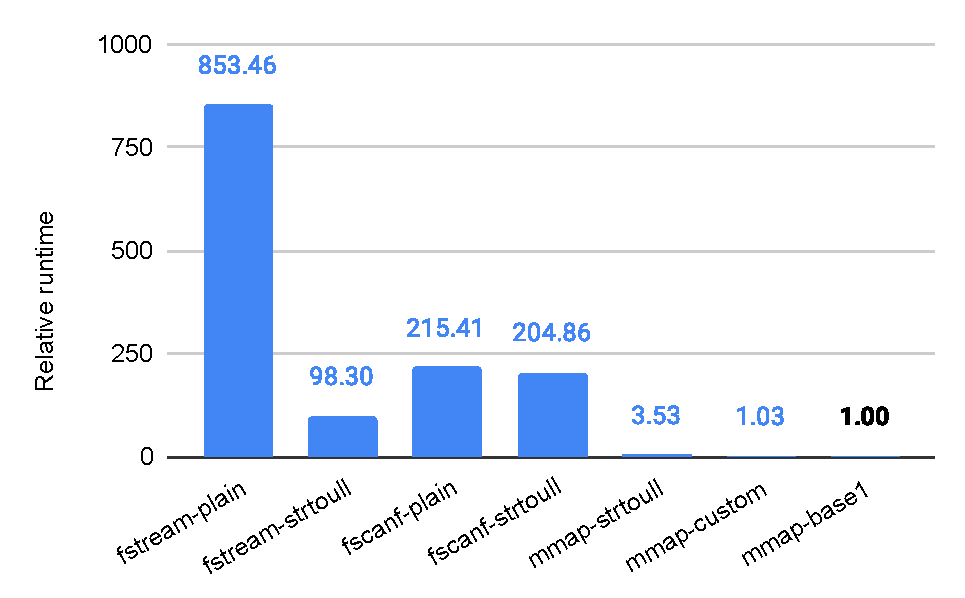
\includegraphics[width=0.99\linewidth]{out/optimize-el.pdf} \\[-2ex]
  \caption{Gini coefficient of PageRank values on 24 different graphs, comparing between PageRank values obtained with three different dead-end handling strategies: \textit{teleport from dead-ends} (\textbf{default}), \textit{self-loop dead-ends} (\textbf{loop}), and \textit{self-loop all vertices} (\textbf{loopall}).}
  \label{fig:optimize-el}
\end{figure}

\begin{figure}[hbtp]
  \centering
  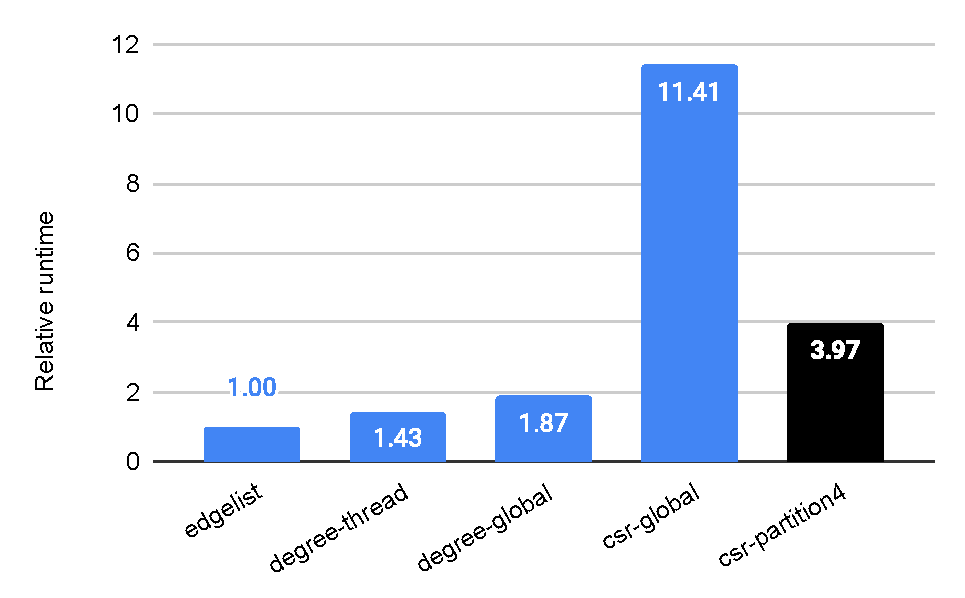
\includegraphics[width=0.99\linewidth]{out/optimize-csr.pdf} \\[-2ex]
  \caption{Gini coefficient of PageRank values on 24 different graphs, comparing between PageRank values obtained with three different dead-end handling strategies: \textit{teleport from dead-ends} (\textbf{default}), \textit{self-loop dead-ends} (\textbf{loop}), and \textit{self-loop all vertices} (\textbf{loopall}).}
  \label{fig:optimize-csr}
\end{figure}



\subsubsection{Results}

Results, shown in Figures \ref{fig:de-gini} and \ref{fig:de-lorenz-all}, indicate that web graphs in general (except \verb|web-NotreDame|) have high Gini coefficient (i.e., high inequality) along with a social network \verb|soc-Epinions1|, and a citation network \verb|cit-Patents|. Road networks are observed to have the lowest Gini coefficient (i.e., low inequality) among all graph classes. If we take a look at the average Lorenz curve of all graphs, we observe that $50\%$ of popularity (ranks) is owned by $\approx20\%$ of the vertices. However, on the web-Stanford graph $50\%$ of popularity is owned by only $\approx3\%$ of vertices, and on the \verb|arabic-2005| (another web graph) is owned by only $\approx1\%$ of the vertices. This would be a significantly worrying level of inequality if each vertex represented a unique person. However, it is possible that many low-ranked pages are low-effort ones and thus have a high page-to-person ratio.

On the social network \verb|soc-Epinions1|, $50\%$ of popularity is owned by only $\approx7\%$ of vertices (Gini coefficient of $\approx0.66$), but on the \verb|wiki-Talk| (a communication graph) $50\%$ of popularity is owned by $\approx46\%$ of vertices (Gini coefficient of $\approx0.07$). This is quite interesting, given that wiki users are usually not ranked, while search engines always rank web pages. Road networks, such as \verb|germany_osm|, are observed to have have a distribution similar to that of \verb|wiki-Talk|.
% Future work could focus on studying the variation of the Lorenz curve and Gini coefficient of various graphs over time.




\subsection{Converting Edgelist to CSR}

In this experiment we study the minimization of Gini coefficient of PageRank values on a number of graphs, using six different deterministic heuristics for adding edges to the graph. First, the PageRank of each vertex is computed in the original graph, and the original Gini coefficient is obtained. A heuristic is then run to obtain the most suitable edge to be added. After this edge is added, the same heuristic is run again. For each heuristic $1000$ edges are added. We plot the variation of Gini coefficient with each added edge for each heuristic.

Our first heuristic, \textbf{edgeInsertCxrx}, adds an edge between the highest contributing vertex to the lowest rank vertex. The idea behind this heuristic is to provide the highest possible increase in rank to the lowest rank vertex. We obtained the highest contributing vertex by finding the vertex with highest $R/(d+1)$ value.

The second heuristic called \textbf{edgeInsertCxSx} is based on the idea of providing the highest possible increase in rank to a vertex which directly or indirectly links to many other vertices (so that it increases the rank of a large number of other vertices as well). This is achieved by adding an edge from the highest contributing vertex to the vertex with highest reverse PageRank. Here, the reverse PageRank of a vertex is obtained by reversing (transposing) the graph, and calculating the PageRanks.

The third heuristic called \textbf{edgeInsertCxSr} is an extension of \textbf{edgeInsertCxSx}, and it prioritizes increasing the rank of vertices which link (directly or indirectly) to a large number of vertices having a low PageRank score. This is done by calculating a modified reverse PageRank, that prioritizes contribution from vertices with low forward PageRank. Here, the reverse rank of each vertex is calculated as $r_u = \alpha R_u r_v / d_v + (1-\alpha)/N$, where $r_u$ is the reverse rank of a given vertex and $R_u$ is its forward rank (precomputed), $r_v$ is the reverse rank of a target vertex and $d_v$ is its in-degree, $\alpha$ is the damping factor, and $N$ is the number of vertices in the graph.

The remaining three heuristics \textbf{edgeInsertCRrx}, \textbf{edgeInsert-CRSx}, and \textbf{edgeInsertCRSr} are a variation of the three heuristics mentioned above where the source vertex is chosen such that it minimizes the rank of the highest ranked vertex. That is, we choose the source vertex with highest contribution to the highest rank vertex. The idea is to reduce rank of high-ranked vertices and increase the rank of low-ranked vertices at the same time, thus reducing inequality.


\subsubsection{Results}

\ignore{It is observed that web graphs tend to have the highest inequality (Gini coefficient), while road networks tend to have the lowest.}As shown in Figure \ref{fig:im-all}, results indicate that the heuristics usually succeed in reducing inequality on graphs with high Gini coefficient (such as web graphs and social networks), but mostly fail on graphs with low Gini coefficient (such as road networks and collaboration networks). It is also observed that the rate of decrease in Gini coefficient decreases as more and more edges are added to graph. In general, we observe that the heuristics \textit{edgeInsertCxrx}, \textit{edgeInsertCxSx}, and \textit{edgeInsertCxSr} perform the best, with \textit{edgeInsertCxSx}, and \textit{edgeInsertCxSr} performing almost identically. \textbf{edgeInsertCxrx} and \textbf{edgeInsertCxSx} heuristics would therefore be the best choices, given that \textit{edgeInsertCxSr} requires a modified PageRank computation.

Based on these results, a suitable approach to minimizing inequality would be to apply both the \textit{edgeInsertCxrx} and \textit{edgeInsertCxSx} heuristics and choose the the best among them for each edge addition. Future research work can include exploring randomized heuristics or looking for better deterministic heuristics.

\begin{figure*}[hbtp]
  \centering
  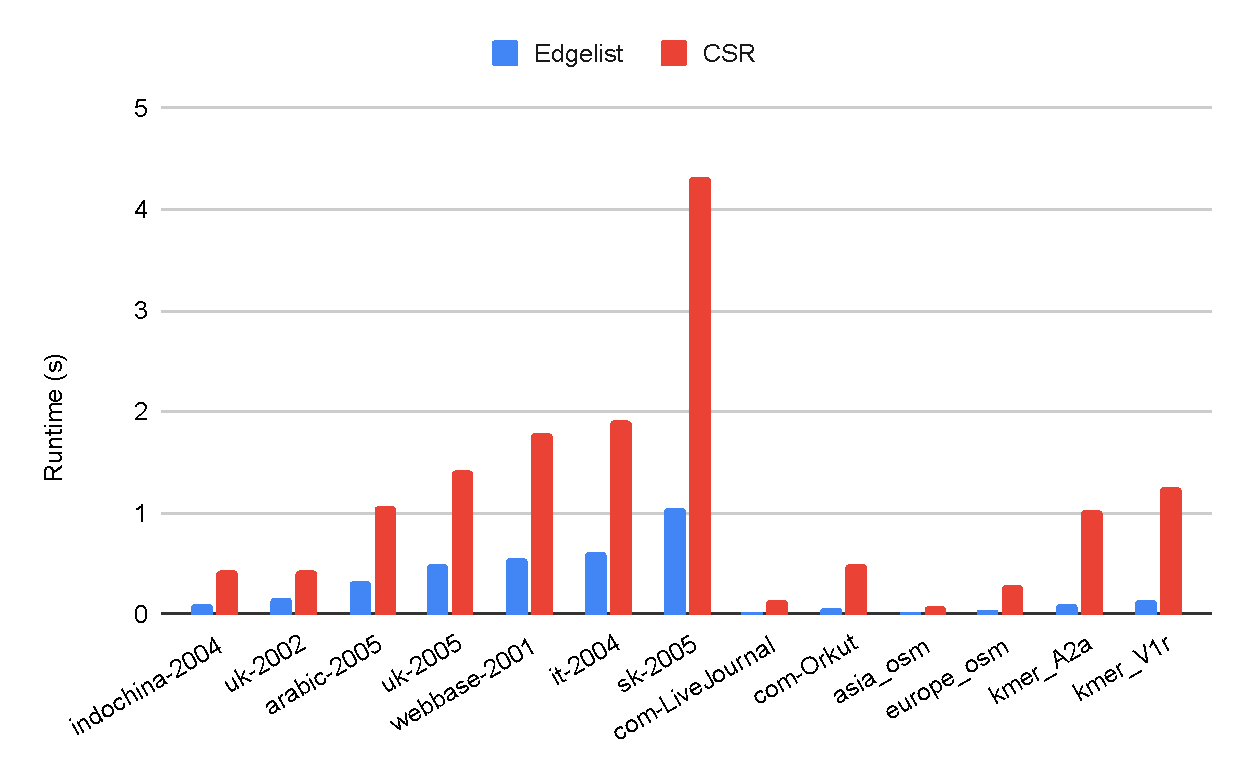
\includegraphics[width=0.68\linewidth]{out/runtime.pdf} \\[-2ex]
  \caption{Time taken by GVEL for edge-list and CSR loading on 13 different graphs.}
  \label{fig:runtime}
\end{figure*}

\begin{figure*}[hbtp]
  \centering
  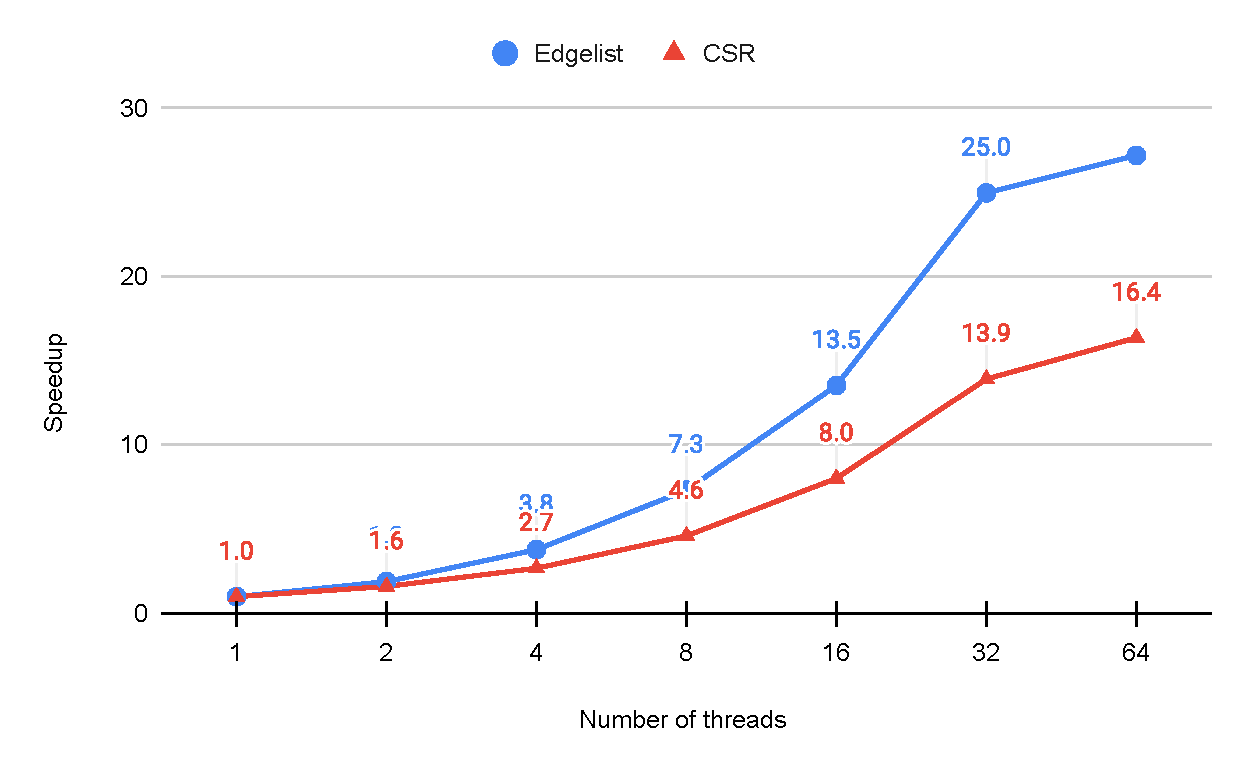
\includegraphics[width=0.68\linewidth]{out/scaling.pdf} \\[-2ex]
  \caption{Speedup of GVEL's Edgelist and CSR loading with increasing number of threads.}
  \label{fig:scaling}
\end{figure*}

\begin{figure*}[hbtp]
  \centering
  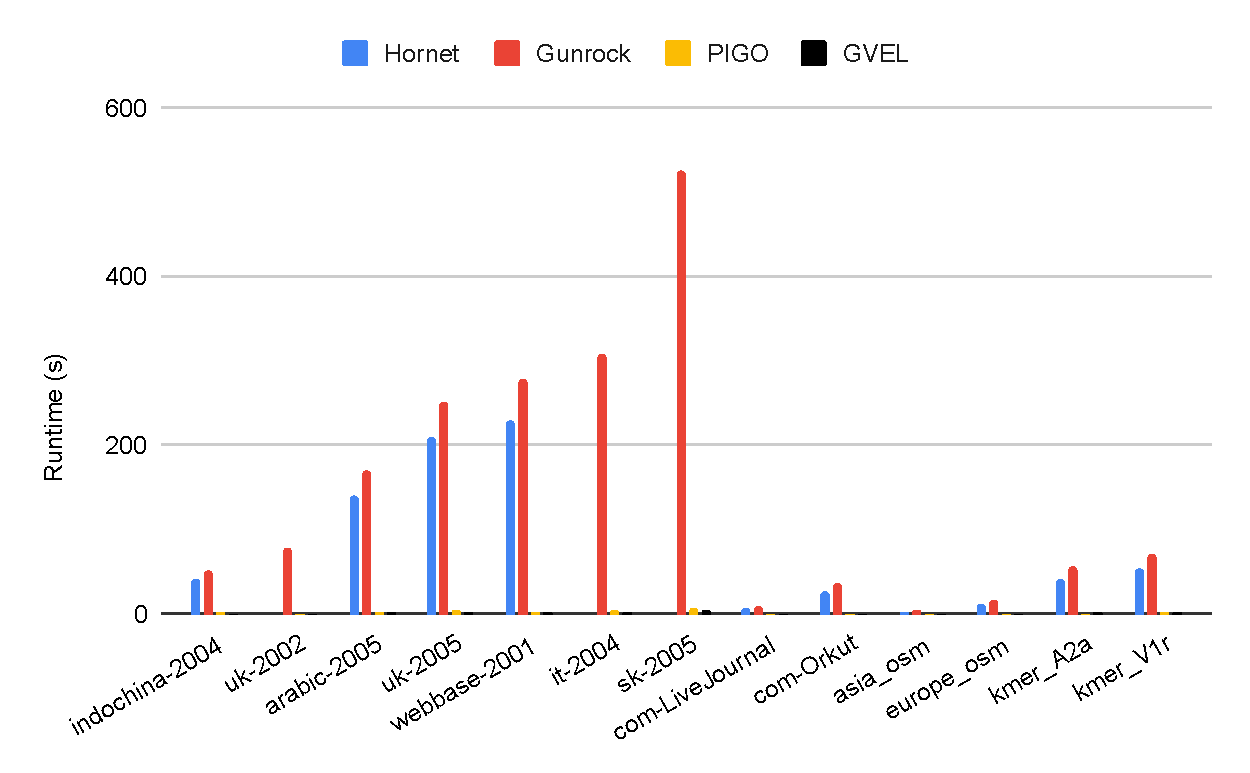
\includegraphics[width=0.68\linewidth]{out/compare-large.pdf} \\[-2ex]
  \caption{Time taken by Hornet, Gunrock, PIGO, and GVEL for reading edge-list and converting it to CSR on 13 different graphs. PIGO and GVEL are not visible on this scale - they are significantly faster than Hornet and Gunrock. The graph loading time for Hornet is not shown for \textit{uk-2002}, \textit{it-2004}, and \textit{sk-2005} graphs as it crashed while loading.}
  \label{fig:compare-large}
\end{figure*}

\begin{figure*}[hbtp]
  \centering
  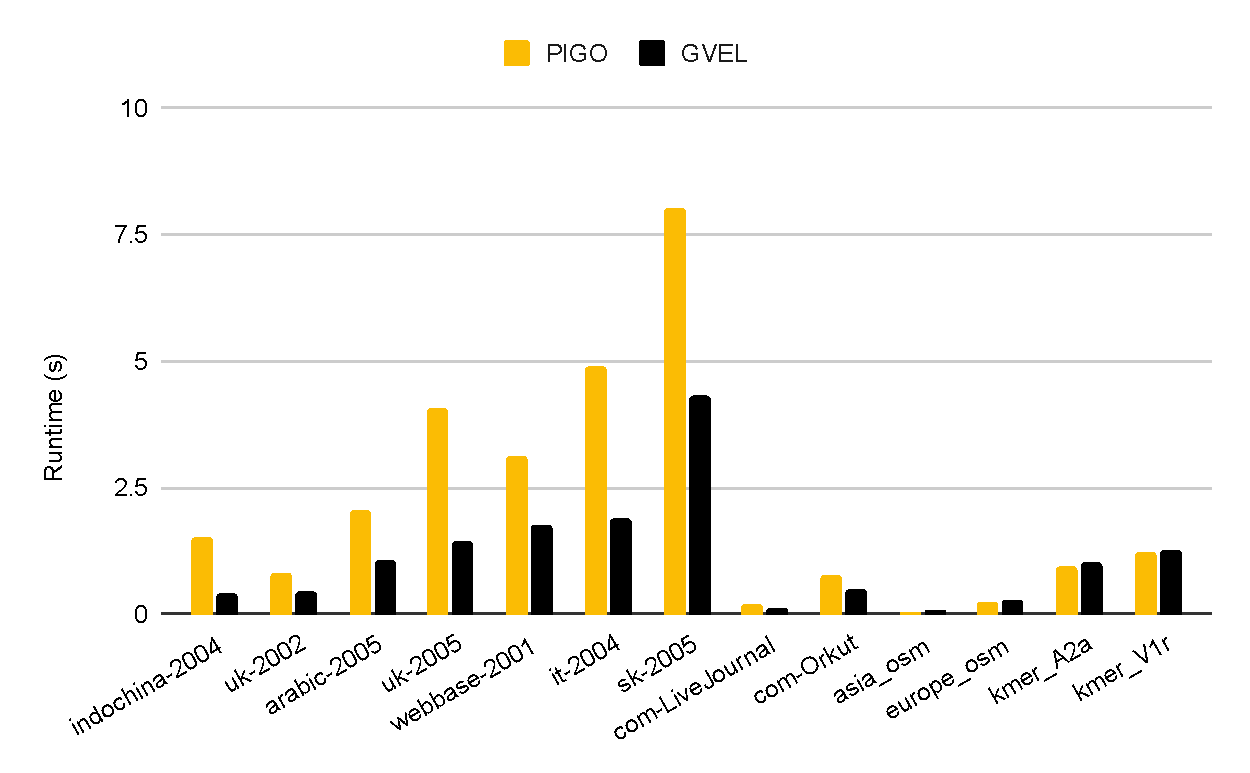
\includegraphics[width=0.68\linewidth]{out/compare-small.pdf} \\[-2ex]
  \caption{Gini coefficient of PageRank values on 24 different graphs, comparing between PageRank values obtained with three different dead-end handling strategies: \textit{teleport from dead-ends} (\textbf{default}), \textit{self-loop dead-ends} (\textbf{loop}), and \textit{self-loop all vertices} (\textbf{loopall}).}
  \label{fig:compare-small}
\end{figure*}

